\chapter{Detector Design and Construction Organization}
\label{vl:tc-overview}

The \dword{dune} \dword{fd} construction project refers collectively 
to the activites associated with the design and construction of the
necessary detector components.  \dword{dune} collaboration management 
is responsible for overseeing this portion of \dword{lbnf-dune} and 
ensuring its successful execution.  The high-level \dword{dune} 
collaboration management team consisting of the co-spokespersons, 
\dword{tcoord}, and \dword{rcoord} is responsible for the
management of the project.  

\section{DUNE Consortia}
\label{sec:consortia}

Construction of the \dword{dune} \dwords{fd} is carried out by 
``consortia of collaboration institutions'' who assume responsibility 
for detector subsystems.  Each consortium plans and executes the 
construction, installation and commissioning of its subsystem.

Management of each consortium is through an overall consortium leader 
and a technical lead.  The consortium leader chairs an institutional 
board composed of one representative from each of the collaborating 
institutions contributing to the activities of the consortium.  Major 
consortium decisions such as technology selections and assignment of 
responsibilities within the institutions are expected to be passed 
through its institutional board.  These decisions are then passed 
as recommendations to the \dword{dune} \dword{exb}, as described in 
greater detail below, for formal collaboration approval.

Figure~\ref{fig:DUNE_consortia_org} shows an example consortium 
organizational chart incorporating the basic structures mandated 
by \dword{dune} Collaboration management.  In addition to the pieces 
described above, consortia in most cases need to manage the design 
and construction of subsystem deliverables that are supported by 
multiple funding agencies.  In the sample case illustrated here, 
responsibilities for subsystem deliverables are shared between the 
USA, UK, and Switzerland (CH), where each of the funding agencies 
is expected to manage its own internal projects with responsibility 
for different sets of assigned deliverables.  To ensure coordination 
between the separate internal projects contributing to the consortia, 
technical leads are responsible for chairing consortium project 
management boards incorporating separate managers from each of 
the internal projects.   
\begin{dunefigure}[DUNE Internal Consortia Structure]{fig:DUNE_consortia_org}
  {\dword{dune} Internal Consortia Structure}
  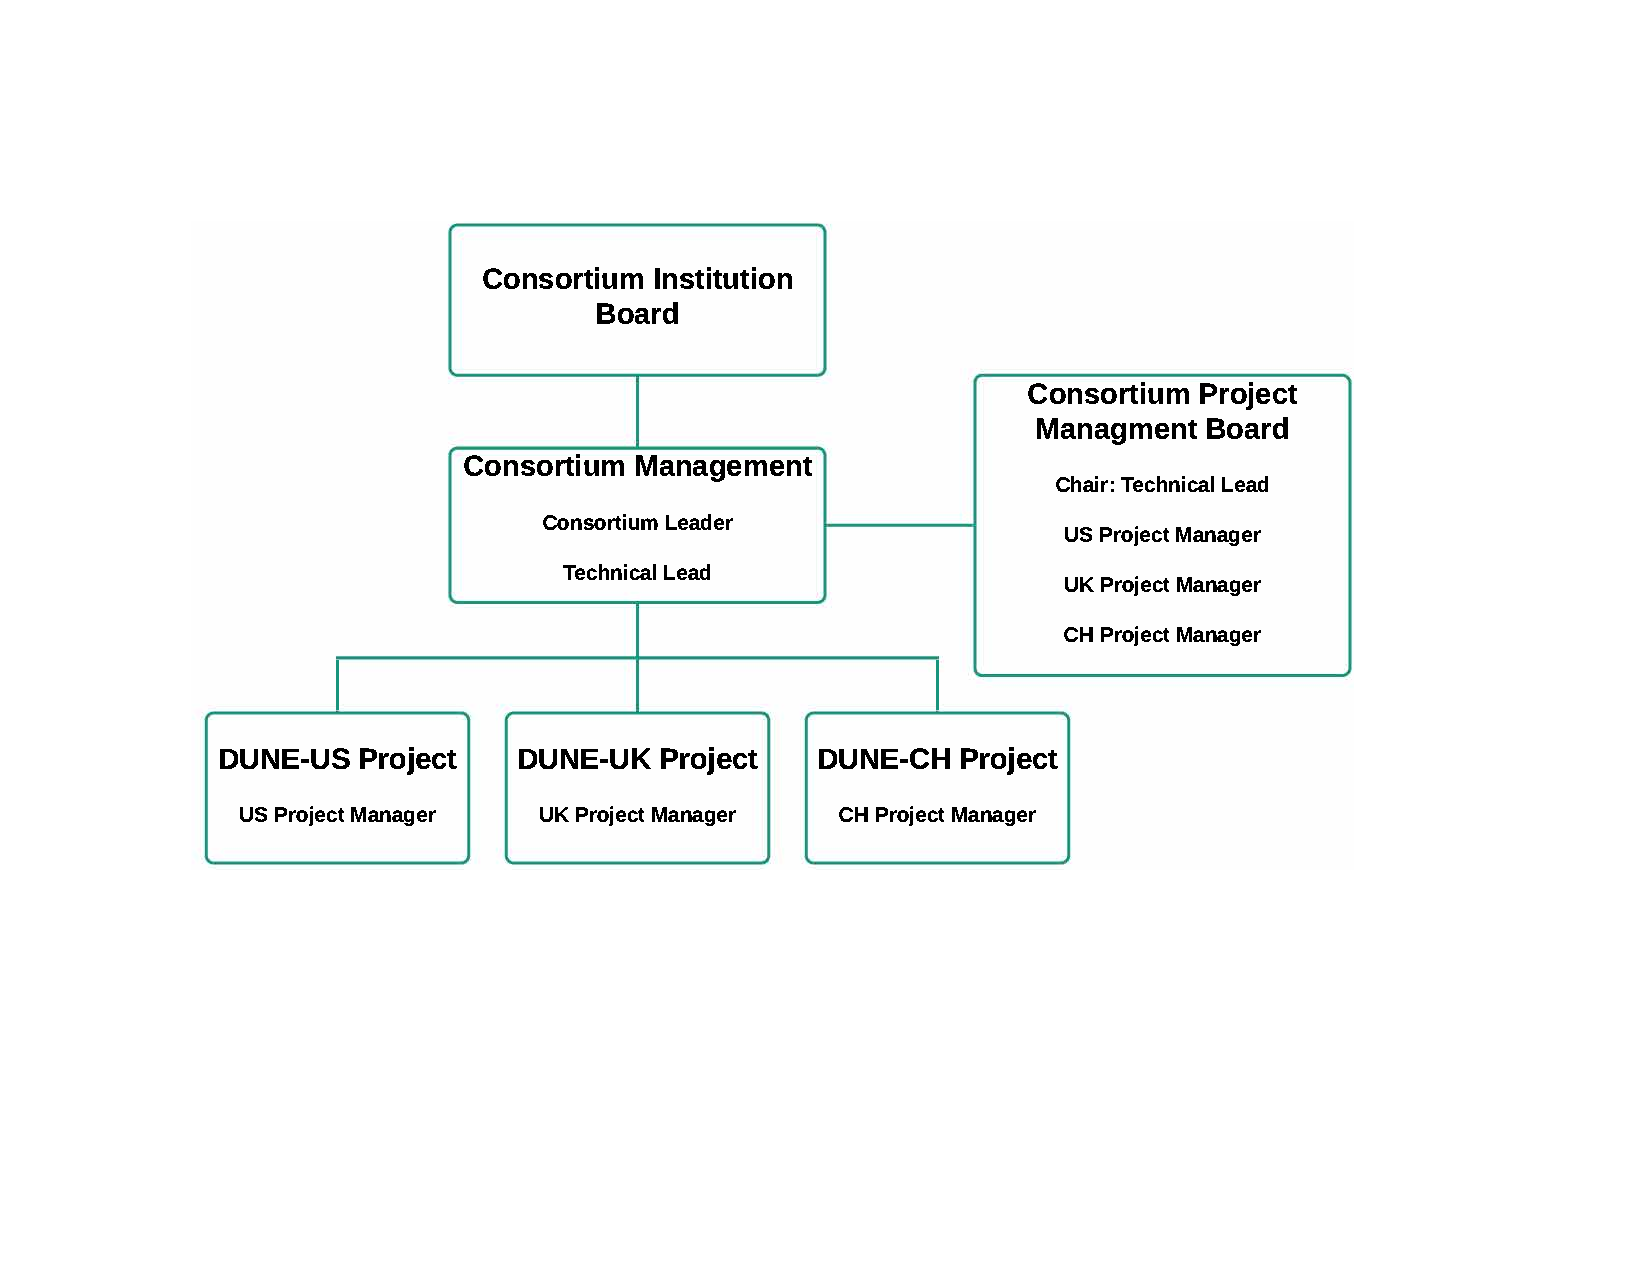
\includegraphics[width=0.99\textwidth]{Internal_Consortia_OrgChart}
\end{dunefigure}

In addition to the mandated organizational pieces described here, 
the consortia incorporate additional internal structures as needed 
to deliver their assigned subsystems.  For example, working groups 
with convenors are typically appointed to focus on specific consortium 
activities, and steering committees are in many cases formed to help 
guide technical and strategic decisions within the consortia.  Each 
consortium is also expected to appoint both safety and \dword{qa} 
representatives as well as a representative with responsibility for 
integration and installation issues.  These individuals are charged 
with interacting directly with the appropriate project support team 
personnel to ensure coordination in these areas across the consortia.        

\section{DUNE Collaboration Management}
\label{sec:dune_mgmt}

The high-level \dword{dune} collaboration management structure is 
shown in Figure~\ref{fig:DUNE_org}.  The \dword{dune} \dword{exb} is 
the primary collaboration decision-making body and as such includes 
representatives from all major areas of activity within the 
collaboration.
\begin{dunefigure}[DUNE org chart]{fig:DUNE_org}
  {\dword{dune} Organizational Chart}
  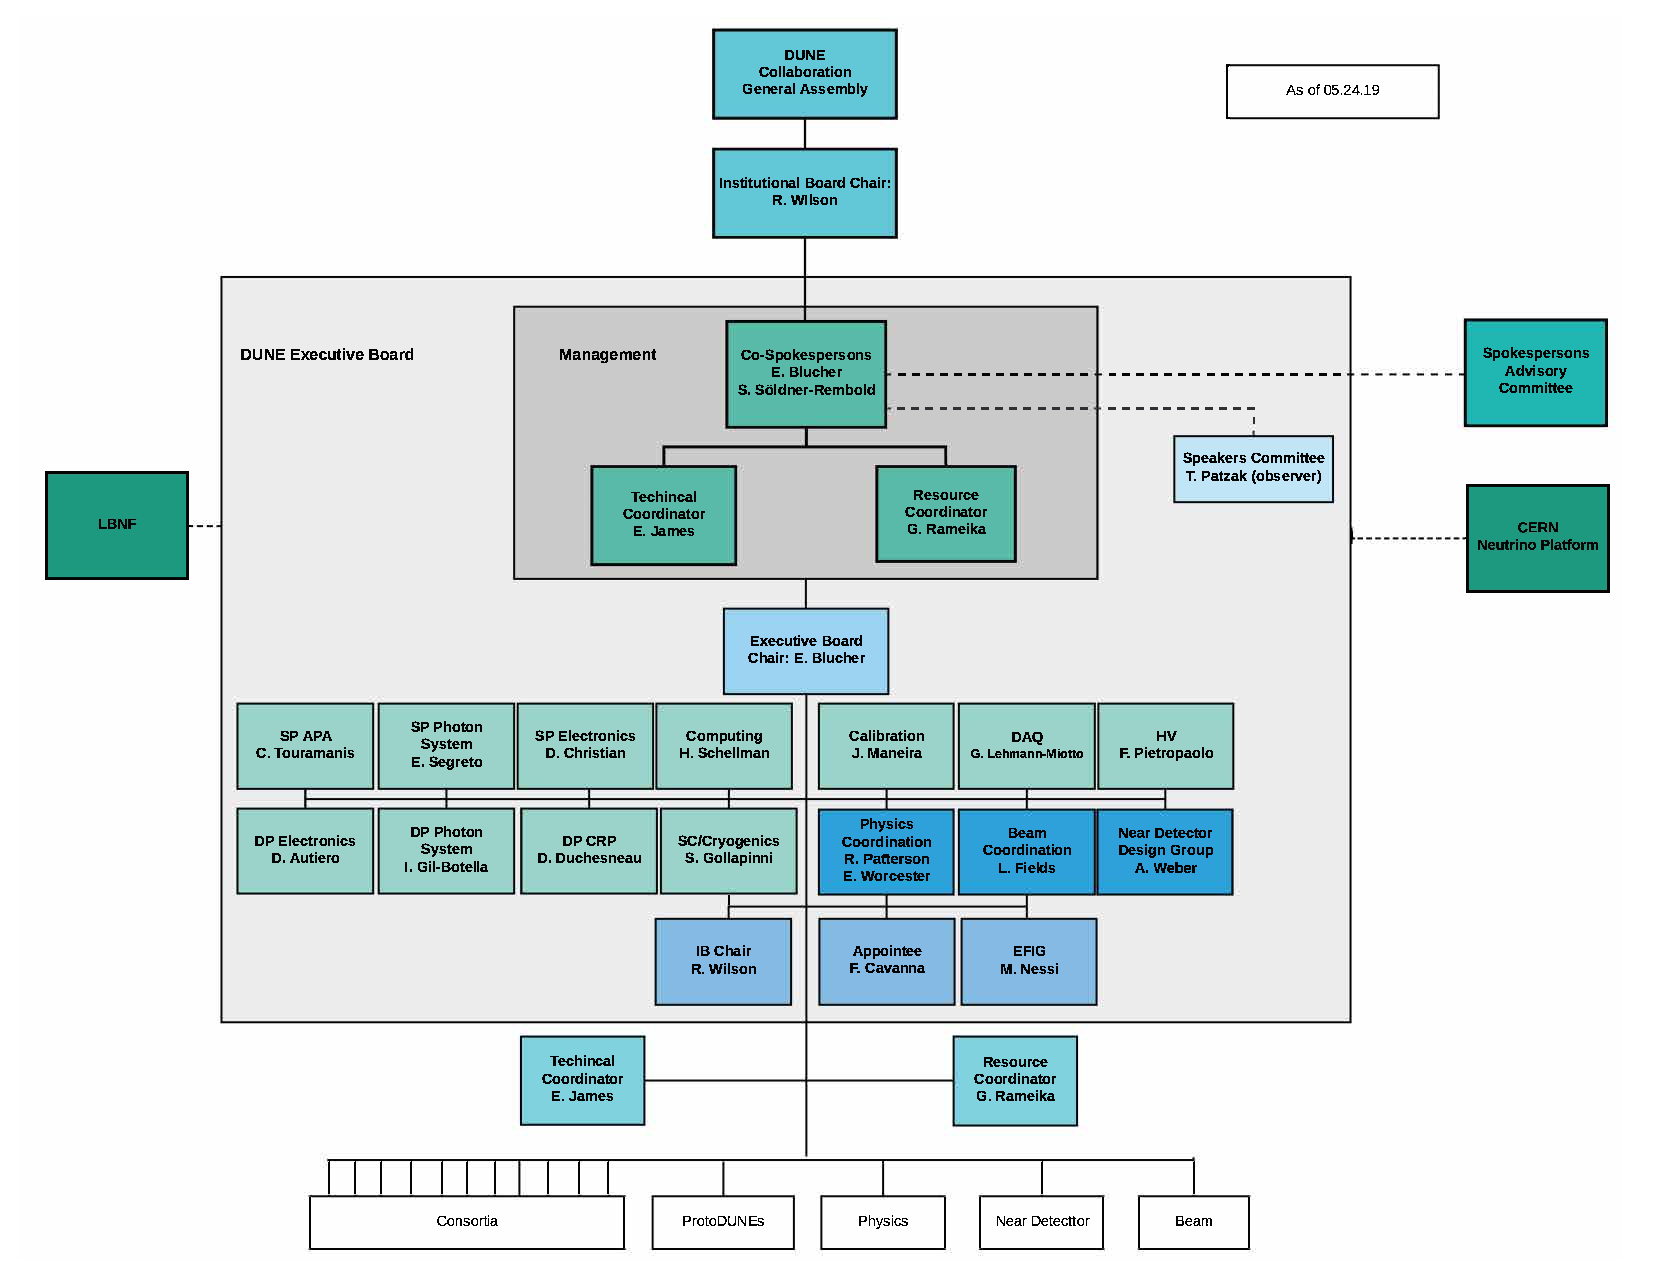
\includegraphics[width=0.95\textheight,angle=90]{DUNE_CollabMgmt_20190525}
\end{dunefigure}
%\fixme{text in boxes should be made bigger}

Each consortium is represented on the \dword{dune} \dword{exb} by its 
consortium leader.  All collaboration decisions, especially those with 
potential impacts on the \dword{dune} scientific program or connected 
with the assignment of institutional responsibilities, pass through the 
\dword{exb}.  \dword{exb} decisions are expected to be achieved through 
consensus.  In cases where consensus cannot be obtained, decision-making 
responsibility passes to the co-spokespersons.

\section{Technical Coordination}
\label{sec:tc}

Because the consortia operate as self-managed entities, a strong
\dword{tc} organization is required to ensure overall integration 
of the detector elements and successful execution of the detector
construction project.  \dword{tc} areas of responsibility include 
general project oversight, systems engineering, \dword{qa}, and 
safety.  \dword{tc} also supports the planning and execution 
of integration and installation activities at \dword{surf} (see 
Chapter~\ref{sec:tco}).  

\dword{tc} is headed by the \dword{tcoord}, who is a \dword{fnal}
employee and is appointed jointly by the \dword{fnal} director 
and the \dword{dune} co-spokespersons.  A deputy \dword{tcoord} 
is selected from within the collaboration to assist the 
\dword{tcoord} in carrying out their responsibilities.

The \dword{tcoord} manages the overall detector construction project
through regular board meetings with the consortium leadership teams 
and members of the \dword{tc} organization (see Section~\ref{sec:tco}).  
These board meetings are used to identify and resolve technical issues
and serve as the primary forums for required interactions between the 
consortia.

Technical board meetings are used to evaluate consortia design
decisions with potential impacts on overall detector performance,
ensure that interfaces between the different subsystems are well
understood and documented, and monitor the overall construction
project to identify and address both technical and interface 
issues as they arise.

Project board meetings are used to ensure that the scopes of 
each consortium are fully documented with assigned institutional
responsibilities, develop and manage risks held within a global
project registry, review and manage project change requests, and
monitor the status of the overall detector construction schedule.

Any decisions generated through these board meetings are passed to the
\dword{dune} \dword{exb} as recommendations for formal approval.
Depending on the agenda items to be discussed at a specific board
meeting, the \dword{tcoord} will invite additional members of the
collaboration with specific knowledge or particular expertise to
participate.  In addition, for major decisions, the \dword{tcoord}
will officially appoint internal collaboration referees with no direct
conflicts of interest to directly engage in the process of evaluating
the technical issues behind these major decisions.

\section{Technical Coordination Organization}
\label{sec:tco}

The \dword{tcoord} heads an organization that supports the work of 
the consortia and has responsibility for a number of major project 
support functions prior to delivery to \dword{surf} including:
\begin{itemize}
\item ensuring that each consortium has a well defined and complete
  scope, that interactions between consortia are sufficiently 
  well defined, and that any missing scope outside of the 
  consortia is provided through other sources such as collaboration
  common funds;
\item defining and documenting scope boundaries and technical 
  interfaces both between consortia and with \dword{lbnf};  
\item developing an overall schedule with appropriate dependencies
  between activities covering all phases of the project. 
\item ensuring that appropriate engineering and safety standards 
  are developed, understood, and agreed to by all key stakeholders 
  and that these standards are conveyed to and understood by each
  consortium;
\item ensuring that all \dword{dune} requirements on \dword{lbnf} 
  for \dword{cf}, cryostat and cryogenics are clearly defined and 
  agreed to by each consortium;
\item ensuring that each consortium has well developed and reviewed
  component designs, construction plans, \dword{qc} processes, and 
  safety programs; and
\item monitoring the overall project schedule and the progress of 
  each consortium towards delivering its assigned scope. 
\end{itemize}

The \dword{dune} \dword{tc} organizational structure is shown 
in Figure~\ref{fig:DUNE_tc}.  The structure incorporates teams 
with responsibilities towards project coordination, detector 
integration, and installation support.  Many \dword{tc} team 
members are also embedded within the \dword{jpo} team (shown 
in Figure~\ref{fig:DUNE_jpo}) in order to ensure coherency in 
these activities across \dword{lbnf-dune}.
\begin{dunefigure}[DUNE Technical Coordination org chart]{fig:DUNE_tc}
  {\dword{dune} \dword{tc} Organizational Chart}
  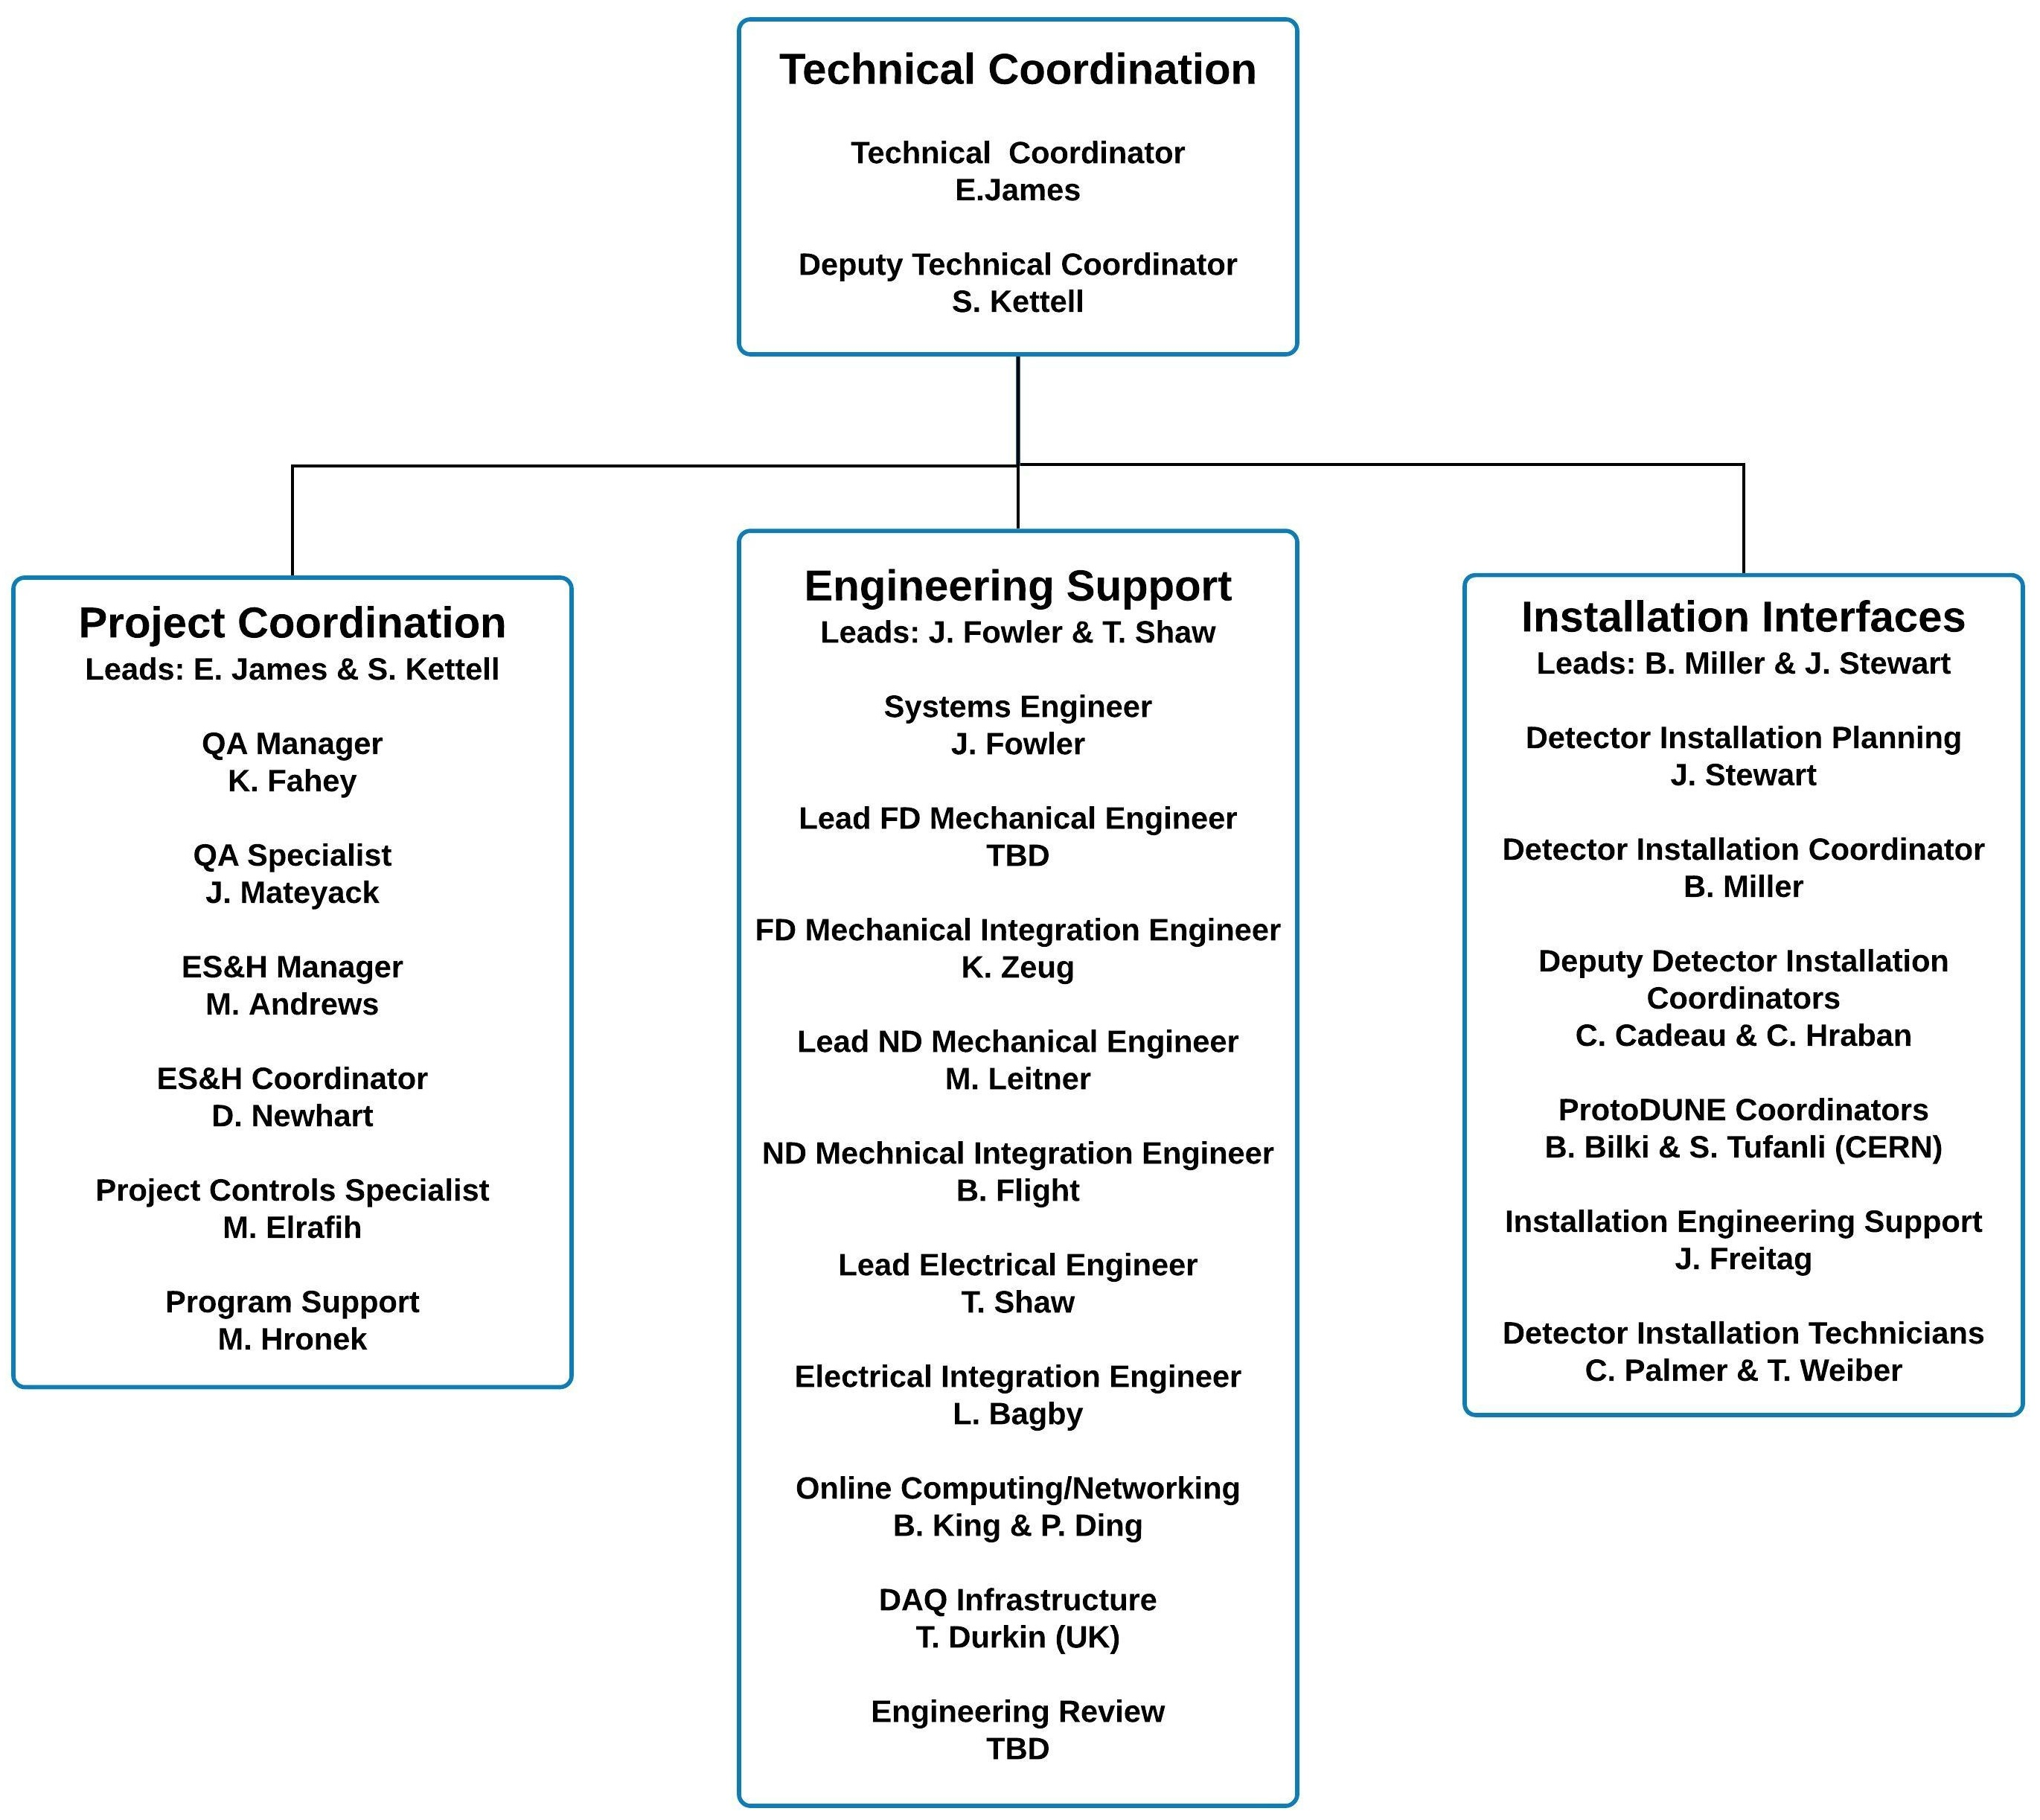
\includegraphics[width=0.99\textwidth]{TC_OrgChart_v2}
\end{dunefigure}
 
The \dword{tc} project coordination team incorporates \dword{esh}, 
\dword{qa}, and project controls specialists.  Engineering support 
is provided through the \dword{tc} detector integration team 
headed by the lead \dword{dune} mechanical and electrical engineers.
Planning coordinators for integration and installation activities 
at \dword{surf} are embedded within both the \dword{jpo} and the 
\dword{tc} installation planning team.  The dual placement of 
these individuals within both organizations facilitates required 
coordination of the integration and installation planning 
efforts between the core team directing these activities and the 
\dword{dune} consortia, which maintain primary responsibility for 
the individual detector subsystems.  Members of the \dword{tc} 
organization meet weekly to review project progress and discuss 
technical issues. 
     
Within the framework of the \dword{dune} \dword{fd} construction 
project, \dword{tc} project support functions associated with its 
coordination role include the following:

\subsection{Safety}

The \dword{tcoord} is responsible for implementing the safety program
covering the \dword{dune} construction project.  The \dword{tcoord}
is supported directly in this role by the \dword{lbnf-dune} \dword{esh}
manager.  A dedicated \dword{dune} \dword{esh} Coordinator sits within
the \dword{tc} organization and guides the \dword{dune} safety program 
under the direction of the \dword{lbnf-dune} \dword{esh} manager.

The \dword{dune} construction project is carried out at many different
institutions in many different countries.  Participating institutions
sign a \dword{mou} in which they agree to abide
by the requirements of the \dword{dune} safety program.  Each of the
participating institutions assumes primary responsibility for the safe
execution of their assigned construction activities.  The \dword{dune}
\dword{esh} coordinator interacts directly with all participating
institutions to ensure that their programs comply with \dword{dune}
safety requirements.  Prior to the start of any construction 
activities, the \dword{dune} \dword{esh} coordinator participates in 
\dwords{prr} incorporating onsite visits to confirm 
that approved safety controls are in place.  Follow-up onsite visits 
by the \dword{dune} \dword{esh} coordinator, including \dwords{ppr}, over the course of the 
construction period are used to validate continuing compliance with
program requirements.

\subsection{Engineering Integration}

\dword{dune} \dword{tc} works directly with the collaboration to 
collect and validate requirements associated with the \dword{fd} 
modules.  Each detector module has its own set of high-level 
requirements with potential impacts on the \dword{dune} physics 
program, which are owned by the \dword{dune} \dword{exb}.  Any 
proposed changes to these requirements must be approved by the 
\dword{exb}.  Lower-level technical requirements associated 
with each detector subsystem are developed by the consortia 
under the guidance of the \dword{tc} detector integration team.  
Appendix~\ref{sec:fdsp-coord-requirements} contains tables 
summarizing the high-level requirements associated with each of 
the \dword{fd} modules.

Starting from these requirements, the \dword{tc} engineering
team responsible for detector integration works directly with the
\dword{dune} consortia to build and validate integrated detector
models from the designs of the individual subsystems.  The team
ensures that the detector subsystems fit together properly and
that the fully-assembled detectors meet structural requirements
associated with all operational conditions (both warm and cold).
The team is also responsible for validating that the integrated
detector designs satisfy the defined requirements needed to meet
the goals of the \dword{dune} physics program.

Integration of the full detector models within the global model
encompassing the detector caverns and supporting infrastructure
is carried out through direct interactions with the \dword{jpo}
engineering integration team.  The \dword{tc} engineering team
is responsible for validating interfaces within the combined
model between \dword{dune} detector components and supporting 
infrastructure pieces.  All proposed changes to the global model 
require approvals from the \dword{tcoord} based on guidance
received from the lead engineers embedded within the \dword{tc}
detector integration team.

As part of these efforts, the engineering team works directly 
with the consortia leadership teams to develop controlled 
documents describing interfaces between the different detector 
subsystems.  These documents are placed under signature control 
within the \dword{lbnf-dune} document management system.  
Proposed changes to interface documents must be approved by 
the consortia leadership teams on both sides of the interface 
as well as by the lead engineers sitting within the \dword{tc} 
detector integration team.

The \dword{tc} engineering team works directly with the
\dword{lbnf-dune} systems engineer, who heads the \dword{jpo} 
engineering integration team, to develop required documents 
detailing interfaces between the \dword{lbnf} and \dword{dune} 
\dword{fd} construction projects and the interfaces of these 
projects with \dword{lbnf-dune} installation and integration
activites at \dword{surf}.  These \dword{lbnf-dune} interface 
documents are also placed under signature control within the 
\dword{lbnf-dune} document management system and proposed 
changes require approvals from both the lead \dword{lbnf-dune} 
systems engineer and the responsible individuals associated 
with each branch of the global project (\dword{lbnf} project 
manager, \dword{dune} \dword {tcoord}, and \dword{ipd}).

Appendix~\ref{sec:fdsp-coord-interface} contains a table 
cataloging the different \dword{dune} interface documents 
and providing web links for accessing the approved versions 
of each in place at the time of the release of this document.
 
\subsection{Change Control and Document Management}

The \dword{dune} project follows the \dword{lbnf-dune} change 
control process described in Section~\ref{sec:fdsp-change}.  
The decision path for changes not impacting the \dword{lbnf} 
project or \dword{lbnf-dune} integration and installation 
activities at \dword{surf} is self-contained within the 
\dword{dune} Collaboration management structure.  A hierarchy 
of decision-making levels is defined based on pre-determined 
thresholds related to the extent of the proposed change 
with the most significant changes requiring \dword{dune} 
\dword{exb} approval.

For document management, the \dword{dune} construction project 
relies on the \dword{lbnf-dune} document management system 
administrated by the \dword{jpo} team configuration manager.  
\dword{tc} works directly with the \dword{lbnf-dune} \dword{qa} 
manager to ensure that the information needed to track the 
history of each detector component through construction, 
assembly and testing is properly captured within the PBS 
database.  A dedicated \dword{dune} \dword{qa} Specialist 
sits within the \dword{tc} organization and coordinates the 
\dword{dune} \dword{qa} program under the direction of the
\dword{lbnf-dune} \dword{qa} manager.  The \dword{dune} 
\dword{qa} program is described in much greater detail in 
Chapter~\ref{vl:tc-QA}.
 
\subsection{Schedule and Milestones}

The lead project controls specialist within the \dword{tc} team works
directly with the \dword{dune} consortia to build schedules covering
the design, testing, and construction activities associated with their
subsystems and incorporate these within the \dword{lbnf-dune}
schedule.  The project controls specialist communicates with consortia
Technical Leads on a monthy basis to track the status of activities
and update the \dword{lbnf-dune} schedule accordingly.  Milestones
positioned at regular intervals within the subsystem construction
schedules are incorporated to enable high-level tracking of these
efforts.  Section~\ref{sec:fdsp-coord-controls} (in
Appendix~\ref{ch:tc-sp-project}) contains a table summarizing key
detector milestones around which the the individual consortia
schedules are constructed.

\subsection{Risk Management}

\dword{dune} \dword{tc} maintains a global registry containing both
subsystem-specific risks identified by the consortia and self-held
risks associated with the overall coordination of the \dword{dune} 
construction project.  The \dword{tcoord} uses Project Board Meetings 
to regularly review the risk registery with the consortia leadership 
teams and define mitigation actions as necessary to prevent identified 
risks from being realized.  The \dword{tcoord} does not have direct 
control over contingency funds held by the internal projects of 
the participating funding agencies.  In cases of identified need, 
the \dword{tcoord} works directly with the consortia leadership teams 
to implement risk reduction strategies.  Identified issues that cross 
consortia boundaries are discussed at Project Board Meetings and 
brought to the \dword{dune} \dword{exb} if they need to be addressed 
at a higher level.

Appendix~\ref{sec:fdsp-coord-risks} contains tables summarizing the 
highest-level identified risks within the \dword{tc} risk registry.

\subsection{Review Process}

The \dword{tcoord} has primary responsibility for conducting design
and production readiness reviews covering each detector subsystem.
As described in Section~\ref{sec:dune_review}, reviews are coordinated
through the \dword{jpo} to ensure coherency across the entire review
process.  The deputy \dword{tcoord} sits within the \dword{jpo} team
responsible for organizing the reviews.  The full review process is
described in greater detail within Chapter~\ref{vl:tc-review}.

\section{DUNE Work Flow}
\label{sec:workflow}

Table~\ref{tab:responsibility} lists the time-ordered set of activities 
required to realize the \dword{dune} \dword{fd} modules, from the design 
of individual detector compnents through operation of the fully-assembled 
modules.  Primary responsibility for the detector subsystems is held 
by the \dword{dune} consortia over the full course of these activities.
\dword{dune} \dword{tc} under the direction of the \dword{tcoord} is 
responsible for coordinating the consortia efforts related to the design, 
prototyping, fabrication, and transport (to South Dakota) of the required 
detector elements.  Efforts related to the receipt (in South Dakota), 
processing, installation, and check out of detector components are coordinated 
through the \dword{jpo} under the direction of the \dword{ipd} as 
described in Chapter~\ref{ch:tc-jpo}.  The \dword{jpo} also coordinates 
efforts related to the installation and commissioning of the supporting
cryogenic infrastructure, for which the \dword{lbnf} project has direct 
responsibility.  The \dword{dune} Collaboration takes responsibility 
for coordinating activities occuring after the cryostats are filled 
with liquid argon beginning with final commissioning of the detectors 
and continuing into long-term detector operation.
\begin{dunetable}
  [DUNE responsibility matrix]
  {|p{0.125\linewidth}|p{0.125\linewidth}|p{0.125\linewidth}|p{0.125\linewidth}|p{0.125\linewidth}|p{0.125\linewidth}|}
  {tab:responsibility}
  {Responsibility matrix for activities occuring during each phase of
   the process for implementing the \dword{dune} \dword{fd} modules.}
               & \dword{dune} & \dword{dune} & \dword{dune}  &             &              \\ 
\rowtitlestyle  Phase        & Consortia    & \dword{tc}   & Collaboration & \dword{jpo} & \dword{lbnf} \\ \toprowrule
  Design       & Lead         & Coordinate   & Support       & Support     &              \\ \colhline
  Prototype    & Lead         & Coordinate   & Support       & Support     &              \\ \colhline
  Fabricate    & Lead         & Coordinate   & Support       & Support     &              \\ \colhline
  Ship         & Lead         & Coordinate   & Support       & Support     &              \\ \colhline
  Receive      & Lead         & Support      & Support       & Coordinate  &              \\ \colhline
  Integrate    & Lead         & Support      & Support       & Coordinate  &              \\ \colhline
  Install      & Lead         & Support      & Support       & Coordinate  & Lead         \\ 
               & (Detector)   &              &               &             & (Cryogenics) \\ \colhline
  Commission   &              &              & Support       & Coordinate  & Lead         \\ 
  (Cryogenics) &              &              &               &             &              \\ \colhline
  Commission   & Lead         &              & Coordinate    & Support     & Support      \\ 
  (Detector)   &              &              &               &             &              \\ \colhline
  Operate      & Lead         &              & Coordinate    &             &              \\ 
\end{dunetable}

Although the organizations responsible for coordinating activities during 
each of stage of the time-ordered process required to bring the \dword{fd} 
modules online are clearly delineated in Table~\ref{tab:responsibility},
there are additional, important support roles connected with each stage.  
The \dword{jpo} interacts with \dword{dune} \dword{tc} during detector 
design, prototyping, and construction to ensure that detector elements 
integrate properly within the supporting infrastructure.  Participation 
of the consortia in the planning process for integration and installation
activities at \dword{surf} is facilitated through \dword{dune} \dword{tc}.
The \dword{dune} collaboration also provides direct support throughout 
the entire process.  The collaboration is responsibile for defining the 
\dword{dune} science program and performing the physics studies used to 
define detector requirements.  The collaboration also provides resources 
that support acquisition of common detector infrastructure items sitting 
outside the scope of the consortia as well as necessary personnel and 
equipment to support integration and installation efforts at \dword{surf}.
\begin{dunetable}
  [DUNE decision-making matrix]
  {|p{0.2\linewidth}|p{0.2\linewidth}|}
  {tab:responsibility2}
  {Responsibility matrix for high-level decision-making occuring during each 
phase of the process for implementing the \dword{dune} \dword{fd} modules}
  & \\
  \rowtitlestyle  Phase             & Decision-making          \\ \toprowrule
  Design            & DUNE EB \\ \colhline
  Prototype         & DUNE EB  \\ \colhline
  Fabricate         & DUNE EB \\ \colhline
  Ship              & DUNE EB  \\ \colhline
  Receive           & EFIG            \\ \colhline
  Integrate         & EFIG     \\ \colhline
  Install           & EFIG      \\ \colhline
  Commission - Cryo & EFIG     \\ \colhline
  Commission - Det  & DUNE EB  \\ \colhline
  Operate           & DUNE EB  \\ 
\end{dunetable}

During each stage of the time-ordered process defined to implement the 
\dword{fd} modules, issues may arise requiring high-level decisions 
on steps required for moving forward.  Table~\ref{tab:responsibility2} 
summarizes which body within the global project structure (\dword{dune}
\dword{exb} or \dword{efig}) takes responsibility for high-level 
decision-making during each stage of the \dword{dune} \dword{fd} 
construction project.  
         
The \dword{dune} project has already completed an initial round of design 
and prototyping activities culminating in the construction and operation 
of the \dword{protodune} detectors.  Moving forward, the project is 
updating detector component designs to account for lessons learned from 
the \dword{protodune} experience.  Upon finalization of the designs, the 
project will construct first production versions of all components that 
will be installed and operated in a second phase of \dword{protodune} 
operations prior to the start of full-scale production.  The operation 
of the \dword{protodune2} detectors will follow roughly two years after
the end of operations for the corresponding \dword{protodune} detectors.
In a few cases, the production of long lead-time components will need to 
be started in parallel with the operation of first production components 
in \dword{protodune2}.
